\documentclass[11pt]{article}

\usepackage{amsmath}
\usepackage{amssymb}
\usepackage[letterpaper,margin=0.72in,headheight=15pt]{geometry}
\usepackage{array}
\usepackage{booktabs}
\usepackage{fancyhdr}
\usepackage{graphicx}
\usepackage{listings}
\usepackage{microtype}
\usepackage{tabularx}
\usepackage{tikz}
\usepackage{xcolor}
\usepackage[hidelinks]{hyperref}

\hypersetup
{
    pdftitle={ADK Lesson 007: AnalogInput and observable scaling},
    pdfauthor={Kevin Shanahan},
    pdfsubject={Measure a potentiometer and map its raw ADC reading to PWM LED brightness},
    pdflang={en-US}
}

\usetikzlibrary{arrows.meta,positioning}
\graphicspath{{docs/lessons/assets/}{../assets/}}

\definecolor{ink}{gray}{0.125}
\definecolor{soft}{gray}{0.949}
\definecolor{mid}{gray}{0.439}
\definecolor{accent}{gray}{0.188}
\definecolor{codebg}{gray}{0.969}

\pagestyle{fancy}
\fancyhf{}
\lhead{\textsc{ADK field lesson 007}}
\rhead{Observe analog input}
\cfoot{\thepage}
\setlength{\parindent}{0pt}
\setlength{\parskip}{5pt}
\renewcommand{\arraystretch}{1.2}

\lstdefinestyle{adkcpp}
{
    language=C++,
    basicstyle=\ttfamily\small,
    backgroundcolor=\color{codebg},
    frame=single,
    rulecolor=\color{mid},
    columns=fullflexible,
    keepspaces=true,
    showstringspaces=false,
    keywordstyle=\bfseries\color{accent},
    commentstyle=\itshape\color{mid},
    breaklines=true,
    tabsize=4
}

\newcommand{\blankline}{\rule{0.96\linewidth}{0.35pt}}
\newcommand{\checkbox}{\(\square\)}

\newenvironment{checkpoint}[1]
{\begin{center}\begin{minipage}{0.94\linewidth}\textbf{Check --- #1}\par}
{\end{minipage}\end{center}}

\begin{document}

\begin{center}
    {\Huge\bfseries Turn a position into evidence}\\[3pt]
    {\Large Lesson 007: \texttt{AnalogInput} and visible scaling}\\[7pt]
    \textit{Predict $\rightarrow$ measure $\rightarrow$ sample
    $\rightarrow$ scale $\rightarrow$ display}
\end{center}

\begin{center}
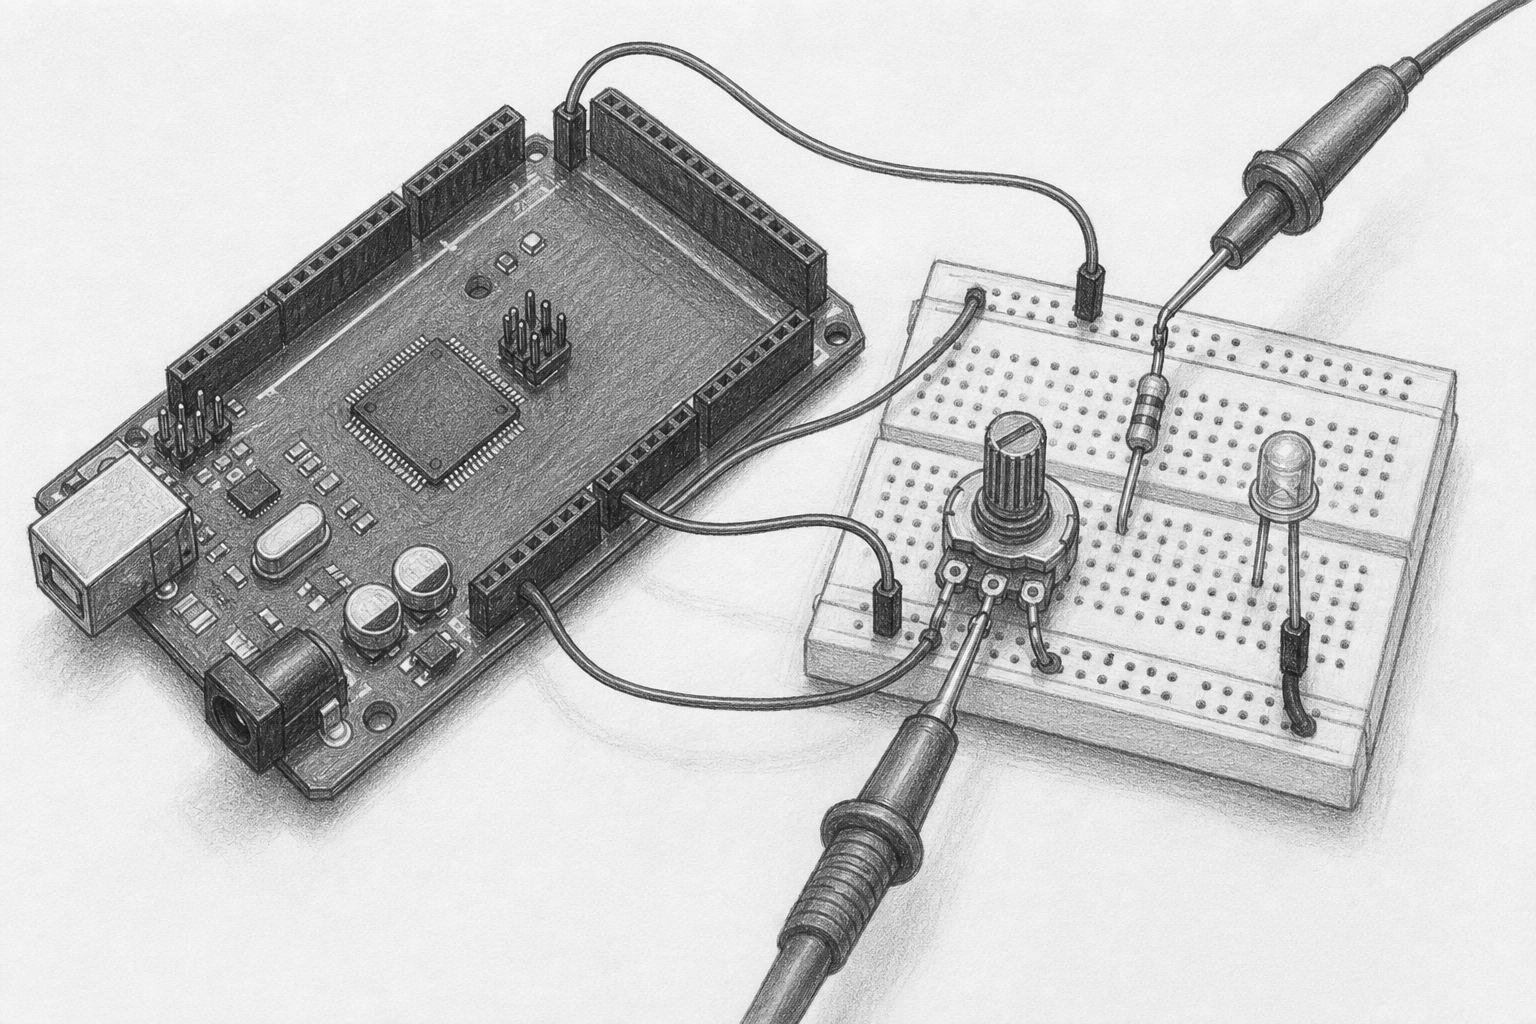
\includegraphics[width=\linewidth,height=0.30\textheight,keepaspectratio]
    {007-analog-input-pencil.png}
\end{center}

\textbf{Orientation plate.}
Use the graphite view to recognize the Mega, potentiometer, LED, and probe
locations. It is not a wiring authority. The exact schematic and connection
table below govern the circuit.

\begin{tabularx}{\linewidth}{@{}>{\bfseries}lX@{}}
Question & Can one raw ADC sample remain observable while an explicit integer
mapping drives PWM brightness?\\
Time & 70--95 minutes\\
Prerequisites & Lessons 001, 004, and the resource-safe lifecycle\\
You need & Mega 2560, USB cable, breadboard, 10\,k\(\Omega\) linear
potentiometer with recorded markings and terminal order, identified LED,
measured 220\,\(\Omega\) resistor, jumpers, multimeter, and logic analyzer or
oscilloscope\\
Evidence & A0 wiper voltage, raw reading, D6 duty waveform, LED brightness,
D13 acquisition indicator, and high-impedance shutdown\\
Safety class & E1: USB-powered Mega, passive potentiometer, and
current-limited LEDs only\\
Status & Host verified; physical acceptance pending\\
\end{tabularx}

\section*{Safety and measurement boundary}

Use only the Mega's USB-derived 5\,V and GND. The potentiometer divides that
same measured supply, which is also the default ADC reference through AVCC; do
not attach an external signal source or drive AREF. Remove USB before changing
any wire. Put meter leads in the correct voltage sockets and clip the black
lead to Mega GND while power is off. Use DC-voltage mode, never current mode.
Before power is applied, record the exact USB source make/model or computer
port, its stated current capability or configured current limit, and the USB
cable identity. Use no unrecorded hub or alternate supply.

\textbf{Stop} for heat, odor, smoke, USB disconnects, an unknown potentiometer
terminal, voltage outside 0--5\,V, or a meter lead in a current jack.
Disconnect USB upstream and inspect the unpowered circuit.
Record the actual LED forward voltage and measured series resistance. At full
duty calculate \(I=(V_{\rm rail}-V_{\rm F})/R\); do not proceed unless the
result is at most 15 mA.

\begin{checkpoint}{before wiring}
\checkbox\ USB removed \quad \checkbox\ resistor measured \quad
\checkbox\ potentiometer terminals identified \quad
\checkbox\ meter in DC-voltage mode
\end{checkpoint}

\section*{1. Read the authoritative circuit}

The potentiometer's outer terminals connect across 5\,V and GND. Its center
wiper is both the A0 input and named test point \textbf{TP-A0}. D6 drives a
separate LED through its own 220\,\(\Omega\) resistor. D13 is the board's
built-in diagnostic LED and consumes one claimed pin.

\begin{center}
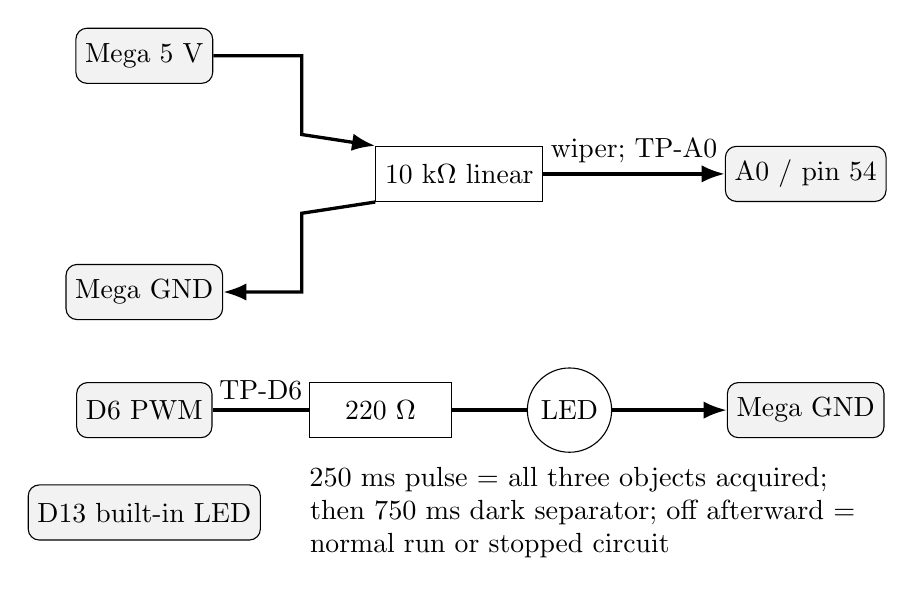
\begin{tikzpicture}[x=1cm,y=1cm,>=Latex,
    terminal/.style={draw,rounded corners,fill=soft,minimum width=17mm,
                     minimum height=7mm},
    part/.style={draw,fill=white,minimum width=18mm,minimum height=7mm}]
    \node[terminal] (vcc) at (0,3.0) {Mega 5 V};
    \node[terminal] (gnd) at (0,0.0) {Mega GND};
    \node[part] (pot) at (4.0,1.5) {10 k\(\Omega\) linear};
    \node[terminal] (a0) at (8.4,1.5) {A0 / pin 54};
    \draw[very thick,->] (vcc)--(2.0,3.0)--(2.0,2.0)--(pot.north west);
    \draw[very thick,->] (pot.south west)--(2.0,1.0)--(2.0,0.0)--(gnd);
    \draw[very thick,->] (pot.east)--node[above]{wiper; TP-A0}(a0);

    \node[terminal] (d6) at (0,-1.5) {D6 PWM};
    \node[part] (r) at (3.0,-1.5) {220 \(\Omega\)};
    \node[draw,circle,minimum size=8mm] (led) at (5.4,-1.5) {LED};
    \node[terminal] (gnd2) at (8.4,-1.5) {Mega GND};
    \draw[very thick,->] (d6)--node[above]{TP-D6}(r)--(led)--(gnd2);

    \node[terminal] (d13) at (0,-2.8) {D13 built-in LED};
    \node[right=5mm of d13,text width=7.0cm] {
        250 ms pulse = all three objects acquired; then 750 ms dark separator;
        off afterward = normal run or stopped circuit};
\end{tikzpicture}
\end{center}

\begin{center}
\begin{tabularx}{0.96\linewidth}{@{}lllX@{}}
\toprule
From & Through & To & Purpose\\
\midrule
Mega 5 V & jumper & potentiometer outer 1 & ADC reference-side terminal\\
potentiometer wiper & TP-A0 & Mega A0 & raw position input\\
potentiometer outer 2 & jumper & Mega GND & common reference\\
Mega D6 & TP-D6, 220\,\(\Omega\) & LED anode & PWM brightness output\\
LED cathode & jumper & Mega GND & output return\\
Mega D13 & built-in circuit & built-in LED & acquisition indication\\
\bottomrule
\end{tabularx}
\end{center}

\textbf{Unpowered proof.} Verify that neither outer potentiometer terminal is
shorted to its neighbor and that the LED path contains the resistor.
Potentiometer rotation direction is not a safety property: swapping only the
two outer terminals reverses the brightness direction.

\section*{2. Predict the evidence chain}

The ADC reports an integer from 0 through 1023. With the default AVCC
reference, one ideal code interval is \(V_{\rm ref}/1024\), so
\[
    \text{reading} \approx
    \min\left(1023,
    \left\lfloor\frac{V_{\rm TP-A0}}{V_{\rm ref}}\times1024\right\rfloor
    \right).
\]
The example maps that raw value to an 8-bit PWM duty:
\[
    \text{duty} =
    \left\lfloor
        \frac{\text{reading}\times255+511}{1023}
    \right\rfloor .
\]
The added 511 rounds rather than always truncating downward. All arithmetic is
unsigned 32-bit so multiplication cannot overflow the AVR's 16-bit
\texttt{int}.

\begin{center}
\begin{tabularx}{0.94\linewidth}{@{}XXXXX@{}}
\toprule
Knob & Predicted TP-A0 & Predicted raw & Predicted duty & Observed\\
\midrule
low & 0.0 V & 0 & 0 & \\
quarter & 1.25 V & 256 & 64 & \\
middle & 2.50 V & 512 & 128 & \\
three-quarter & 3.75 V & 767 & 191 & \\
high & 5.0 V & 1023 & 255 & \\
\bottomrule
\end{tabularx}
\end{center}

Code 1023 therefore represents the top interval below the reference, not an
exact 5.000\,V measurement. Real values vary with measured AVCC, potentiometer
tolerance, contact noise, ADC quantization, converter error, and meter
accuracy. The 10\,k\(\Omega\) potentiometer has at most about
2.5\,k\(\Omega\) Thevenin source resistance, comfortably below the
datasheet's approximately 10\,k\(\Omega\) source-impedance guidance. Lesson
008 will calibrate and filter these measurements. This lesson deliberately
preserves the raw sample.

\section*{3. Read the owning interface}

\texttt{AnalogInput} is inert after construction. Initialization validates and
claims the pin, selects input mode, and caches the first raw reading.
\texttt{update()} performs one new conversion; \texttt{read()} returns that
cached value without silently sampling again.

\begin{lstlisting}[style=adkcpp]
adk::Runtime     runtime;
adk::AnalogInput potentiometer (runtime.resources (), 54);

if (potentiometer.initialize ().ok ())
{
    potentiometer.update ();
    const adk::AnalogInput::Reading raw = potentiometer.read ();
}

potentiometer.shutdown ();
\end{lstlisting}

\texttt{Reading} is \texttt{uint16\_t}; valid values are 0 through
\texttt{AnalogInput::maximumReading} (1023). Pin 54 is Mega A0. Shutdown makes
the pin high impedance, releases its claim, and retains the last cached reading
only as historical software state. A retained number is not a live voltage.

\texttt{PwmOutput} owns D6. Its value is switched duty, not a steady analog
voltage. Shutdown writes zero, selects input mode, and releases its pin and
shared timer lease. \texttt{MonoLed} owns D13 and turns its semantic LED off
before release.

\section*{4. Let the example tell the run-loop story}

The canonical sketch declares the objects in dependency order. Its
\texttt{setup()} acquires the diagnostic LED, input, and output. D13 pulses
for 250 ms only after all three initialize, then remains dark for a 750 ms
separator. Its \texttt{loop()} then reads as the circuit does and reaches
\texttt{stopSafely()} after a fixed 120-second run:

\begin{lstlisting}[style=adkcpp]
potentiometer.update ();
const adk::AnalogInput::Reading position   = potentiometer.read ();
const adk::PwmOutput::Duty      brightness =
    chooseBrightness (position);

if (!brightnessLed.write (brightness).ok ())
{
    stopSafely ();
}
\end{lstlisting}

\textbf{Observe}: take exactly one explicit raw sample and publish
\texttt{raw=<count>,duty=<value>} at 115200 baud whenever it changes.
\textbf{Decide}: map position into the output domain.
\textbf{Actuate}: command one PWM duty. Any command failure tears the whole
circuit down; D13 turns off and both signal pins become high impedance.

The complete, compiled source is
\texttt{examples/Lesson007AnalogInput/Lesson007AnalogInput.ino}. Do not maintain
a second sketch copied from this page.

\section*{5. Build, upload, and observe from the CLI}

No IDE is required. From the repository root:

\begin{lstlisting}[style=adkcpp,language=bash]
make bootstrap
make arduino-Lesson007AnalogInput
make upload EXAMPLE=Lesson007AnalogInput PORT=/dev/ttyACM0
\end{lstlisting}

Use \texttt{make boards} to discover the port. The LED and named test points
remain the primary evidence. Optional records expose the exact raw-to-duty
transformation:

\begin{lstlisting}[style=adkcpp,language=bash]
make monitor-describe PORT=/dev/ttyACM0
make monitor PORT=/dev/ttyACM0 BAUD=115200
make serial-log PORT=/dev/ttyACM0 BAUD=115200 \
    SERIAL_LOG=build/serial/lesson007.log
\end{lstlisting}

Disconnect any monitor before uploading if the operating system cannot share
the port. Serial is supporting evidence and cannot replace circuit
observations.

\section*{6. Predict, observe, interpret}

\subsection*{Resource-acquisition evidence}

\textbf{Predict}: after reset, D13 remains off until every owner initializes,
pulses for 250 ms, then stays off after a 750 ms dark separator.
\textbf{Observe}: capture D13 timing with the logic analyzer or oscilloscope.
\textbf{Interpret}: the pulse supports the claim that the program acquired
A0, D6, and D13. No pulse supports startup failure; it does not identify the
failed owner or prove correct breadboard wiring.

\subsection*{Input evidence at TP-A0}

\textbf{Predict}: with the meter's black lead on Mega GND, TP-A0 moves
continuously from near 0 to near 5\,V as the knob turns.
\textbf{Observe}: measure at low, middle, and high positions.
\textbf{Interpret}: the voltage proves the divider and common reference. It
does not by itself prove which raw integer software cached.

\subsection*{Output evidence at TP-D6}

\textbf{Predict}: the LED is off near raw 0 and grows brighter toward raw 1023;
the optional record contains the corresponding exact raw count and duty.
At middle position, a logic analyzer or oscilloscope shows D6 switching with
about 50\% high time. \textbf{Observe}: compare the LED and TP-D6.
\textbf{Interpret}: the waveform supports correct scaling and PWM command.
A handheld meter may display an average-like value; that reading is not proof
of a steady analog voltage.

\subsection*{Safe-state evidence}

The canonical sketch calls \texttt{stopSafely()} 120 seconds after the
acquisition sequence. Predict the deadline, capture D6 becoming inactive, and
confirm both LEDs remain off. Then remove USB before moving any lead.

Test A0 and D6 one at a time. With USB removed, disconnect the potentiometer
wiper from A0 for the A0 test, then connect the selected pin to the midpoint
of two 10\,k\(\Omega\) resistors placed in series from 5 V to GND. Inspect the
fixture, restore USB, and measure the midpoint relative to the named Mega GND.
A reading near one-half the measured rail supports high impedance; a value
near a rail contradicts it. Remove USB before moving the fixture from A0 to
D6 or restoring the normal circuit. Never open the ground connection or move
a bare probe while powered. The midpoint test, not LED darkness, is the
safe-state evidence.

\section*{7. Diagnose by following the evidence}

\begin{center}
\begin{tabularx}{\linewidth}{@{}p{0.23\linewidth}p{0.34\linewidth}X@{}}
\toprule
Observation & Most useful next check & What it separates\\
\midrule
D13 never pulses & remove power; inspect pin choices and unpowered continuity &
initialization/resource failure from the run loop\\
D13 on, TP-A0 fixed & probe wiper, then both outer terminals relative to GND &
divider wiring from software mapping\\
TP-A0 varies, LED fixed off & inspect LED polarity/resistor; then probe TP-D6 &
load wiring from PWM command\\
LED changes backward & swap the two outer potentiometer terminals while
unpowered & orientation from correctness\\
LED flickers near one position & hold the knob; record TP-A0 stability &
contact/sample noise from mapping defects\\
TP-D6 appears ``2.5 V'' & observe with a logic analyzer or oscilloscope &
PWM average indication from a steady voltage\\
\bottomrule
\end{tabularx}
\end{center}

\section*{8. Deterministic host proof}

The host fake supplies exact ADC readings; no test sleeps or depends on a
physical knob. Required cases cover 0, 1, 511, 512, 1022, and 1023; invalid and
non-analog pins; resource conflict; repeated initialization and shutdown;
destruction while active; failed setup rollback; and pin reuse after release.
The mapping table is pure integer arithmetic, so the same raw trace yields the
same duties on every run.

\begin{lstlisting}[style=adkcpp,language=bash]
make host-test
make host-test-exceptions
make quality
\end{lstlisting}

These commands prove software contracts and compilation, not the physical
Mega circuit.

\section*{9. Bench acceptance card}

\begin{tabularx}{\linewidth}{@{}>{\bfseries}lX@{}}
Board / revision & \\
USB source / port / stated current capability or limit & \\
USB cable identity & \\
Measured Mega 5 V rail & \\
Arduino CLI / AVR core & \\
Potentiometer markings / terminal order & \\
LED package / color / polarity & \\
Resistor marked / measured value & \\
LED forward voltage / calculated active current & \\
Meter make / model / mode & \\
Analyzer or oscilloscope / probe & \\
10 k\(\Omega\) fixture resistors, measured & \\
Sketch revision & \\
Reviewer / date & \\
\end{tabularx}

\begin{center}
\begin{tabularx}{\linewidth}{@{}p{0.25\linewidth}p{0.21\linewidth}p{0.28\linewidth}X@{}}
\toprule
Claim & Prediction & Observation & Interpretation\\
\midrule
Resources acquired & D13 pulses 250 ms, then 750 ms dark & & \\
Low input & TP-A0 near 0 V; record raw near 0; LED off & & \\
Middle input & TP-A0 near half rail; record duty near 128 & & \\
High input & TP-A0 near rail; record duty 255 & & \\
PWM is switched & TP-D6 toggles at recorded middle duty & & \\
LED current bounded & At duty 255, calculated current is at most 15 mA & & \\
Timed shutdown & At 120 s, TP-D6 stops toggling; LEDs stay off & & \\
A0 released & Separate midpoint fixture reads near half rail & & \\
D6 released & Separate midpoint fixture reads near half rail & & \\
Reset recovers & Reset restarts pulse, separator, and deadline & & \\
Power removed & USB removal makes rail and test points 0 V & & \\
Rollback proof & Host-injected D6 acquisition failure releases A0/D13 & & \\
\bottomrule
\end{tabularx}
\end{center}

\textbf{Acceptance status:}
\checkbox\ not run \quad \checkbox\ pass \quad \checkbox\ deviation recorded

\section*{10. Exercises}

\begin{enumerate}
    \item Calculate expected raw readings from your measured supply and TP-A0
    values. Explain discrepancies without changing code.
    \item Reverse only the two outer potentiometer wires while unpowered.
    Predict the entire evidence table before reconnecting USB.
    \item Change the mapping so the minimum visible duty is 16 while raw zero
    still means off. State the new integer formula and boundary cases.
    \item Change the optional record policy to emit only when raw changes by a
    useful threshold. Explain why this cannot change the circuit-native
    acceptance criteria.
    \item Sketch a calibration object for Lesson 008. Keep sampling,
    calibration, filtering, and PWM ownership as separate responsibilities.
\end{enumerate}

\section*{Use with and next step}

Use the HTML lesson for maintained API links, errata, source downloads, and
copyable commands. Use this PDF at the bench for prediction, measurement,
diagnosis, and the signed acceptance record. Lesson 008 adds calibration,
dead bands, and deterministic filtering. Lesson 009 composes them into an
adaptive night light with explicit sensor-fault states.

\section*{Primary references}

\begin{itemize}
    \item \href{https://docs.arduino.cc/hardware/mega-2560}
    {Arduino Mega 2560 Rev3 documentation and pinout}
    \item \href{https://www.microchip.com/en-us/product/ATmega2560}
    {ATmega2560 datasheet, ADC, and electrical characteristics}
    \item \href
    {https://arduino.github.io/arduino-cli/latest/commands/arduino-cli/}
    {Arduino CLI command reference}
\end{itemize}

\textbf{Deferred evidence.}
The repository records host and compile gates. No physical voltage, waveform,
current, shutdown, reset, or power-removal claim becomes accepted until a
person completes this card on the named Mega 2560 and publishes the result.

\end{document}
